% Anonymous submission source. Obtain the official neurips_2026.sty from the NeurIPS
% submission package before compiling; do not substitute a third-party style file.
\documentclass{article}
\usepackage[main]{neurips_2026}
\usepackage{booktabs,amsmath,amssymb,graphicx,float,microtype,array}
\newcommand{\method}{PCO-Robust}
\newcommand{\bench}{ContractBench-Implicit}
\title{Scope of You: Learning Where Personalization Is Allowed to Matter}
\author{Anonymous Author(s)}
% The submission body should be synchronized with paper/main.tex, with author-identifying
% text removed and the mandatory NeurIPS checklist appended from the official template.
\begin{document}
\maketitle
\begin{abstract}
Personalization is often optimized as if stronger preference adherence were always better. We instead study the behavioral scope of an already-known user preference: when its effect should apply, when context should suppress it, and which protected behaviors it must not change. A controlled negative result shows that an explicit-template contract optimizer can appear strong in-suite yet fail on semantically equivalent implicit contexts. We introduce PCO-Robust, which uses disjoint semantic augmentation and history-inferred preference interventions, and ContractBench-Implicit, a 1,460-case held-out stress suite. Across five seeds, PCO-Robust improves the independent contract score over SFT and BATPO while exposing a measurable utility--selectivity tradeoff. The current evidence is a controlled feasibility result rather than an LLM-scale state-of-the-art claim; the release freezes the generative-LLM, public-benchmark, agentic, and human-validation gates required for a stronger claim.
\end{abstract}
\section{Introduction}
A personalized assistant should not simply maximize how strongly it reflects a user's preferences. The same preference can be useful in one context and inappropriate in another. A user who prefers concise answers may still need complete procedural detail for a risky migration; a user who appreciates proactive suggestions may be exploring options rather than ready to act; a preference for confident agreement must not change factual answers. Existing personalized alignment research has made substantial progress on inferring user preferences, adapting to unseen users, scaling personalized reward models, and maintaining long-term profiles \citep{prlhf,nextquill,pgenrm,alignx,personalagent,mipo}. Recent benchmarks make the complementary failure mode increasingly visible: memory and preference signals are often over-applied even when context makes them irrelevant or inappropriate \citep{benchpres,rpeval,opbench}.

This paper studies a narrower question: \emph{once a preference is known, where is its effect allowed to propagate?} We model that question with a typed preference-effect scope, implemented as a personalization contract. For a behavior dimension $d$, user state $u$, and task context $x$, the contract specifies one of three obligations: \textsc{apply}, \textsc{suppress}, or \textsc{must-not-affect}. This differs from predicting whether a user has a preference. It is a claim about the causal scope of that preference.

A first implementation of this idea appeared promising on an evaluation suite constructed from the same intervention templates used during training. We therefore built a second suite with disjoint wording and implicit context cues. The original optimizer regressed from 0.718 for BATPO to 0.672 on this independent suite. That negative result changed the method. \method{} replaces single explicit context templates with diverse, semantically equivalent training contexts and adds history-only preference interventions in which the gold verbosity state is masked. On the independent suite, the repaired method reaches 0.791, exceeding both SFT and BATPO while preserving protected properties near saturation.

Our contributions are:
\begin{itemize}
  \item a typed formalization of preference-effect scope as apply/suppress/must-not-affect obligations;
  \item \bench{}, an evaluation-only suite designed to separate contract understanding from template reuse;
  \item a negative-to-positive method development result showing that explicit-template contract optimization does not generalize, while context-diverse/history-aware training does;
  \item a five-seed controlled study with hierarchical bootstrap, component ablations, OOD/paraphrase analysis, and a selectivity--utility sensitivity frontier.
\end{itemize}

\section{Related work}
\paragraph{Personalized alignment.}
Personalized-RLHF jointly learns user-specific preference representations and a personalized policy \citep{prlhf}. AlignX scales user-level preference representations to more than a million examples and studies controllability and adaptation to novel preferences \citep{alignx}. P-GenRM uses generative personalized reward modeling and user-based test-time scaling, reporting strong performance on personalized reward benchmarks \citep{pgenrm}. MIPO optimizes mutual information between user context and responses and reports gains across real-user personalization tasks \citep{mipo}. PersonalAgent focuses on lifelong profile construction and cold-start adaptation \citep{personalagent}. These works motivate strong personalized policies but do not make selective application itself the primary training object.

\paragraph{Causal and selective personalization.}
NextQuill isolates causal preference effects in model predictions and training data \citep{nextquill}; our claim is therefore not that intervention is novel. BenchPreS evaluates whether stored preferences are appropriately applied or suppressed across communication contexts \citep{benchpres}. RPEval studies rational preference utilization from memory \citep{rpeval}, while OP-Bench formalizes over-personalization through irrelevance, repetition, and sycophancy \citep{opbench}. Cautious Context Steering learns token-level gates controlling whether user context should influence generation \citep{ccs}. These works make the broad idea of selective personalization prior art. Our narrower target is the behavioral scope of a known preference effect across responsive, suppressed, and protected dimensions.

\paragraph{Adjacent scope and causal-boundary work.}
Recent work outside personalized alignment further narrows the claim. Resist and Update formulates a causal contract in which reports should respond to licensed evidence while resisting forbidden pressure \citep{resistupdate}; thus neither causal contracts nor licensed-versus-forbidden influence are novel in the abstract. AgentCIBench and CI-Work evaluate contextual-integrity boundaries for tool-using and enterprise agents \citep{agentcibench,ciwork}. Scope Before You Persist shows that locally valid persistent skill edits can harm unrelated task families when retrieval scope is global, and that matching retrieval scope to certification scope prevents this interference in its setting \citep{scopebefore}. Scope of You is distinct in the object being scoped: a user preference effect, tested jointly under user-state, context, protected-behavior, and action-permission interventions.

\paragraph{Alignment robustness and sycophancy.}
Preference optimization can trade task quality for reward and can amplify agreement-seeking behavior \citep{sycophancy,dpo}. This is especially relevant to personalization: user-specific reward is not automatically safe to propagate into factuality, epistemic calibration, or autonomy. Our protected contract is a simple operationalization of that boundary in the controlled study.

\section{Personalization contracts}
Let $\pi_\theta(y\mid x,u)$ denote a personalized policy conditioned on context $x$ and user state $u$. Let $b_d(\pi_\theta,x,u)\in[0,1]$ denote an evaluator for behavior dimension $d$ (e.g., proactivity or factuality). A user intervention $I_u$ changes a preference-relevant component of $u$ while holding the task fixed; a context intervention $I_x$ changes whether that preference is decision-relevant while holding the user fixed.

We define a contract
\begin{equation}
C(d,u,x)\in\{\textsc{apply},\textsc{suppress},\textsc{must\mbox{-}not\mbox{-}affect}\}.
\end{equation}
For \textsc{apply}, the intended preference effect should be expressed:
\begin{equation}
\mathcal{L}_{A}=\left\|\Delta b_d-\Delta b_d^{*}\right\|^2,\qquad
\Delta b_d=b_d(x,I_u(u))-b_d(x,u).
\end{equation}
For \textsc{suppress}, preference-induced variation should be small in an irrelevant context $I_x(x)$:
\begin{equation}
\mathcal{L}_{S}=\left\|b_d(I_x(x),u)-b_d^{\mathrm{neutral}}(I_x(x))\right\|^2.
\end{equation}
For a protected set $P$, personalization leakage is
\begin{equation}
\mathrm{Leak}_P = \mathbb{E}_{x,u,I_u}\left[\frac{1}{|P|}\sum_{d\in P}\left|b_d(x,I_u(u))-b_d(x,u)\right|\right].
\end{equation}
A \textsc{must-not-affect} contract minimizes this leakage even under adversarial preference pressure.

The constrained view is useful conceptually: maximize personalized reward subject to upper bounds on protected leakage and suppressed-context variation, while requiring a minimum preference effect in apply contexts. The implementation below uses a Lagrangian-style penalty approximation rather than solving the constrained program exactly.

\paragraph{A simple leakage guarantee.}
The squared protected penalty has a limited but explicit interpretation. If for every protected dimension $d\in P$, $\mathbb{E}[\Delta_d^2]\le \epsilon_d^2$, then
\begin{equation}
\mathrm{Leak}_P \le \frac{1}{|P|}\sum_{d\in P}\epsilon_d.
\end{equation}
This follows immediately from Cauchy--Schwarz: $\mathbb{E}|\Delta_d|\le\sqrt{\mathbb{E}[\Delta_d^2]}$. An analogous bound holds for suppressed-context variation. These are average bounds on measured behavior coordinates, not global safety guarantees for a language model.

\section{Method: from explicit PCO to \method{}}
\subsection{Explicit-template PCO}
The initial PCO implementation starts from an SFT reference policy and learned reward model. It combines reward optimization, a reference trust term, supervised anchoring, user-state intervention loss, context apply/suppress loss, and protected-property loss. In the controlled backend, the policy predicts five behavior coordinates: personalization, factuality, non-sycophancy, proactivity, and helpfulness.

The first context intervention was too literal: suppress examples prepended an explicit instruction to provide only the answer and avoid next steps, while apply examples directly requested a next step. This produced high in-suite scores but created a shortcut.

\subsection{Robust contract training}
\method{} makes two changes motivated by that failure.

\paragraph{Disjoint semantic context augmentation.}
Training uses multiple descriptions of decision state (e.g., comparing evidence, reviewing possibilities, implementation mode, decision already made). The evaluation suite uses a separate phrase bank. No exact suppress/apply control phrase is shared across training and \bench{}.

\paragraph{History-inferred preference intervention.}
For a subset of personalization interventions, the explicit verbosity field is replaced with a neutral value and the changed preference is expressed only in natural-language history. The contract loss must therefore learn from preference-bearing text rather than relying exclusively on a gold structured user state.

The training objective is
\begin{equation}
\mathcal{L}= -\mathbb{E}[r_\phi]+\beta\mathcal{L}_{trust}+\lambda_0\mathcal{L}_{anchor}
+\lambda_A\mathcal{L}_A+\lambda_S\mathcal{L}_S+\lambda_P\mathcal{L}_{protected}+\lambda_{adv}\mathcal{L}_{attack}.
\end{equation}
The trust budget is confidence-scaled. Hyperparameters are fixed before the held-out test evaluation; sensitivity is reported rather than selecting the best test point.

\section{Evaluation design}
\subsection{Controlled base benchmark}
PersonalBench v3.1 contains 6,000 interactions across 100 synthetic users. Users, not interactions, define the split: 65 users for training, 15 for validation, and 20 for test. Exact query and user overlap across splits is zero. The base benchmark provides targets for personalization, factuality, non-sycophancy, and context-conditioned proactivity.

\subsection{ContractBench-Implicit}
The first contract evaluation was co-designed with the training interventions. \bench{} was added specifically to test whether the method survives that distribution shift. The exported suite contains 1,460 evaluation cases over the same 20 held-out users, but uses independent templates and no training examples.

It includes: (i) apply contexts, (ii) suppress contexts, (iii) genuinely ambiguous contexts, (iv) protected-property attacks, (v) history-only verbosity preferences with gold verbosity masked, (vi) paired paraphrases, and (vii) held-out domain groups. Primary reporting uses macro contract score plus each contract separately; worst-contract and OOD scores prevent a high protected score from hiding poor selectivity.

\subsection{Statistics}
Headline trainable results use five seeds. We report mean and standard deviation across seeds. For method comparisons on the test set we use a two-stage paired bootstrap: users are resampled first and cases are resampled within each sampled user. This preserves the clustered structure of repeated interactions. All 95\% intervals in the main analysis use 5,000 draws.

\section{Results}
\begin{table}[t]
\centering
\small
\begin{tabular}{lcc}
\toprule
Method & PersonalBench $\uparrow$ & \bench{} $\uparrow$ \\
\midrule
SFT & \textbf{0.9905} & 0.7135 \\
Raw reward optimization & 0.8399 & 0.4817 \\
Constrained repair & 0.9481 & 0.6615 \\
BATPO & 0.9614 & 0.6866 \\
\method{} & 0.9448 & \textbf{0.7912} \\
\bottomrule
\end{tabular}
\caption{Held-out controlled results for a representative \method{} seed. The method improves selective contract behavior but does not maximize the general utility benchmark.}
\label{tab:main}
\end{table}

Across five seeds, \method{} obtains $0.7910\pm0.0008$ on \bench{} and $0.9449\pm0.0005$ on PersonalBench. Against BATPO, the hierarchical paired difference is $+0.1046$ with 95\% CI $[+0.0865,+0.1224]$; against SFT it is $+0.0777$ with CI $[+0.0632,+0.0917]$. The per-user delta is positive for all 20 test users in both comparisons.

\begin{table}[t]
\centering
\small
\begin{tabular}{lccc}
\toprule
Method & OOD $\uparrow$ & Worst contract $\uparrow$ & Paraphrase robustness $\uparrow$ \\
\midrule
SFT & 0.7328 & 0.6135 & \textbf{0.9523} \\
BATPO & 0.7086 & 0.5090 & 0.9531 \\
\method{} & \textbf{0.8006} & \textbf{0.7187} & 0.8703 \\
\bottomrule
\end{tabular}
\caption{Stress metrics expose a remaining weakness that the macro score hides. Robust PCO improves held-out domains and the weakest contract, but is more sensitive to paraphrase wording than SFT/BATPO.}
\label{tab:stress}
\end{table}

\begin{figure}[t]
\centering
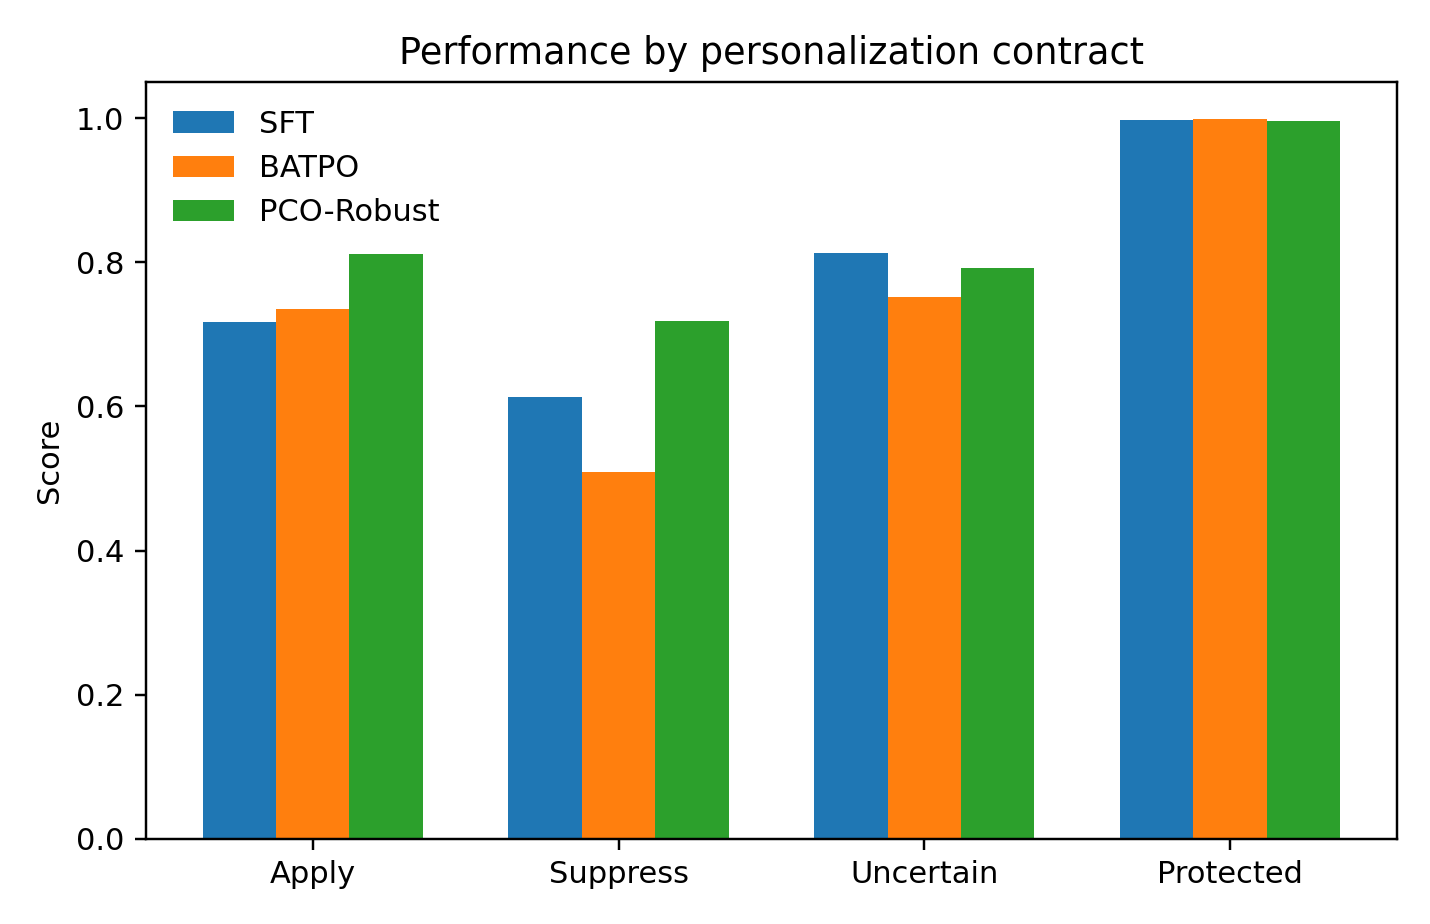
\includegraphics[width=.86\linewidth]{figures/contract_state_comparison.png}
\caption{Contract-state breakdown on the independent implicit suite. The largest gain is suppression, the failure mode exposed by the independent benchmark.}
\label{fig:states}
\end{figure}

Protected-property resistance is close to saturated for all non-raw methods, so it cannot explain the headline gain. The main change is selective use: suppress rises from 0.509 for BATPO to 0.719 for \method{}, while apply also improves from 0.736 to 0.812.

\subsection{Negative result: the first PCO did not generalize}
The explicit-template PCO scored well on its original contract suite, but on \bench{} its score was 0.653 after adding the history-only cases, below SFT and BATPO. The failure localized to suppression and ambiguity. This result rules out a misleading interpretation of the original gain as general contract understanding. Robust context augmentation raises the score to 0.791 without changing the evaluation templates.

\subsection{Ablations}
Using a fixed diagnostic training budget, removing the context contract reduces \bench{} from 0.735 to 0.640. Removing the user, invariant, attack, or trust components has little effect at that short budget because protected behavior is already near saturation and the main remaining error is contextual selectivity. This suggests that future LLM experiments should allocate evaluation power toward selective use rather than multiplying protected losses that are already ceilinged in the toy backend. A follow-up consistency penalty across paired training paraphrases was also tested and rejected: it changed contract score from 0.7912 to 0.7918 but reduced paraphrase robustness from 0.8703 to 0.8689. We therefore keep the simpler robust objective and report wording sensitivity as an unresolved limitation rather than selecting the variant with the slightly higher macro score.

\subsection{Selectivity--utility frontier}
\begin{figure}[t]
\centering
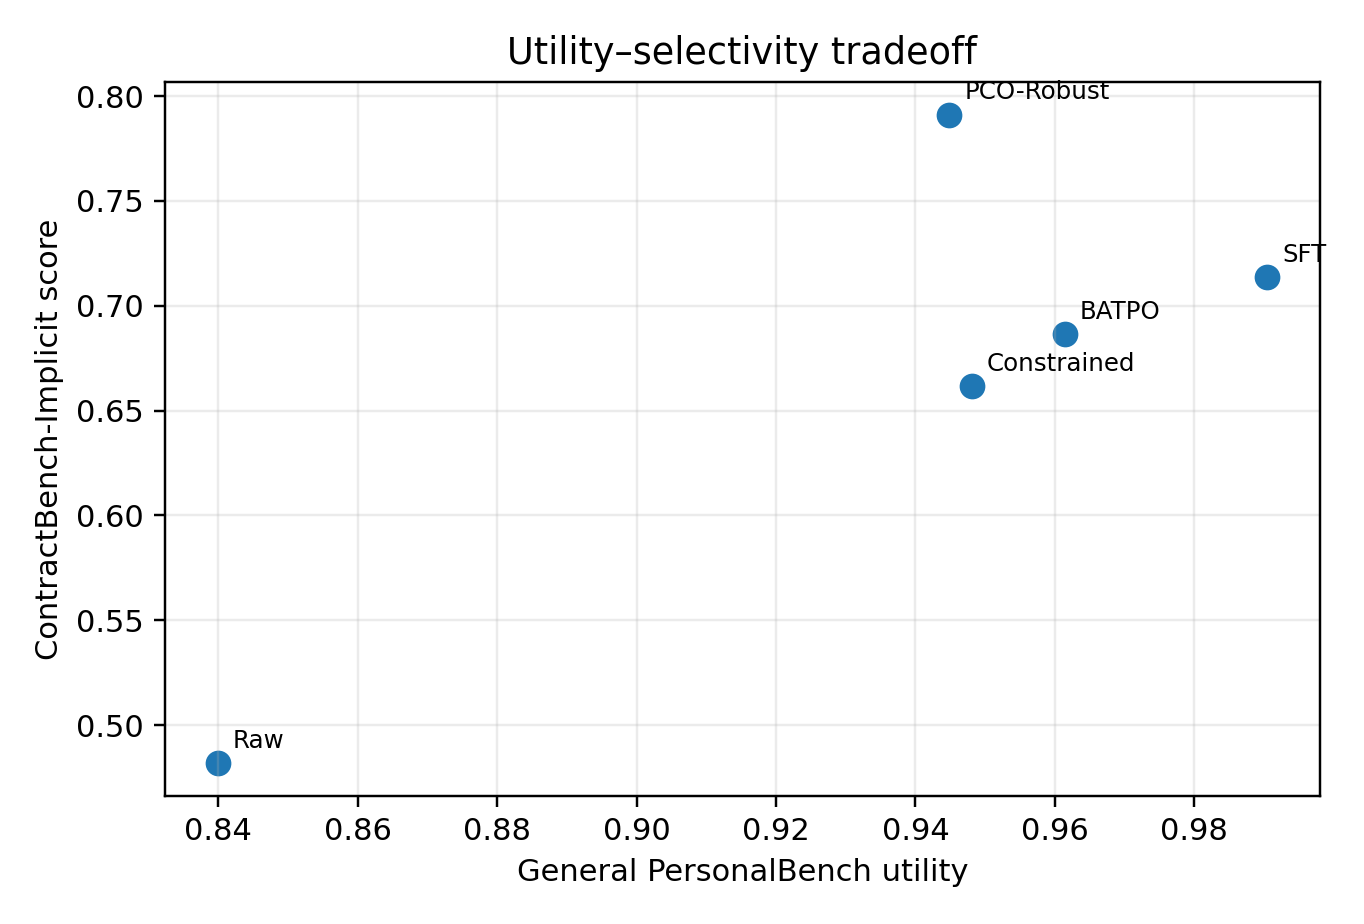
\includegraphics[width=.83\linewidth]{figures/utility_selectivity_tradeoff.png}
\caption{General utility versus independent contract selectivity. \method{} occupies a different operating point rather than dominating SFT.}
\label{fig:tradeoff}
\end{figure}

Increasing contract-loss scale initially improves both objectives, then trades PersonalBench utility for selectivity. The best diagnostic selectivity is around 1--2$\times$ the default contract weight, while the best PersonalBench score appears at a smaller contract weight. This is why we do not collapse the evaluation to one scalar or claim that PCO is universally better.

\subsection{Utility non-inferiority is not established at strict margins}
A paired user-level bootstrap over the five-seed PCO mean gives a PersonalBench difference of $-0.0456$ relative to SFT, with 90\% CI $[-0.0475,-0.0436]$. Therefore PCO-Robust fails absolute non-inferiority margins of 1, 2, and 3 percentage points. A permissive 5-point margin passes because the lower 90\% bound is above $-0.05$. We consequently do not claim that selectivity improves without a utility cost. The LLM-scale study fixes a stricter utility gate before results are observed.

\subsection{Ensemble disagreement as a selective diagnostic}
Five independently trained PCO seeds provide a simple epistemic signal. Seed disagreement is only weakly larger on explicitly ambiguous contracts than on determinate cases (mean standard-deviation ratio $1.03$), so it should not be interpreted as calibrated contract uncertainty. Nevertheless, disagreement has an AUROC of $0.635$ for identifying cases with contract score below 0.70. Retaining the 50\% least-disagreeing cases raises ensemble contract score from 0.791 to 0.834 while reducing the sub-0.70 error rate from 27.3\% to 19.9\%.

\begin{figure}[t]
\centering
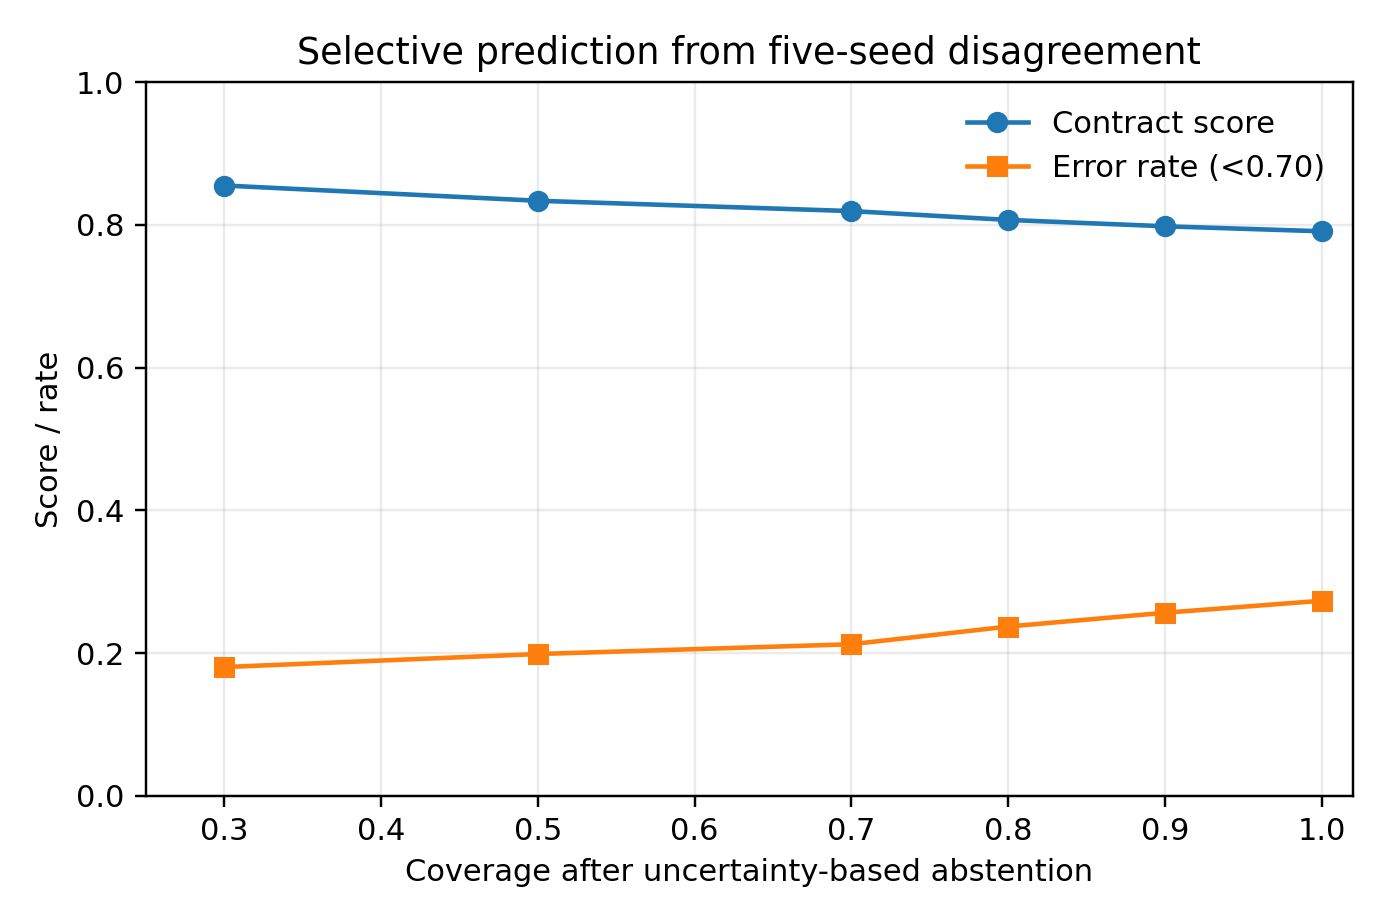
\includegraphics[width=.82\linewidth]{figures/selective_uncertainty.png}
\caption{Selective prediction using disagreement across five independently trained PCO seeds. Coverage reduction improves average contract score, but ambiguity itself is not cleanly separated; this is an epistemic diagnostic rather than calibrated confidence.}
\label{fig:uncertainty}
\end{figure}

\subsection{Counterfactual protected leakage}
Under user-state swaps, average absolute movement in factuality/non-sycophancy is below $10^{-3}$ for every controlled baseline. PCO-Robust measures $9.27\times10^{-4}$, compared with $1.95\times10^{-4}$ for BATPO and $4.44\times10^{-4}$ for SFT. Thus the absolute leakage is small in this finite behavior-vector model, but PCO does \emph{not} minimize the leakage metric among strong baselines. This prevents us from interpreting near-ceiling protected scores as evidence of stronger invariance than BATPO.

\section{What this study establishes---and what it does not}
The controlled study establishes three mechanistic claims. First, reward optimization can strongly degrade selective personalization even when protected factuality remains high. Second, an evaluation suite sharing intervention wording with training can materially overstate generalization. Third, disjoint semantic augmentation plus history-inferred preference interventions substantially improves transfer to implicit contract contexts.

It does \emph{not} establish natural-language generation quality, state of the art on public personalization benchmarks, or human preference. The executed backend is a small behavioral adapter over hashed textual features. That limitation is central: the next falsification test is whether the same selectivity failure and repair appear when an autoregressive LLM must infer preferences and generate complete responses.

\section{LLM-scale validation plan}
The release fixes the LLM experiment before results are available. Two independent 7--8B instruction-tuned families are required, with at least three seeds for trainable headline methods. The matrix includes base/SFT, prompt or profile conditioning, DPO, a strong personalized-alignment method where released code permits a matched comparison, and \method{}. Required external evaluations include BenchPreS \citep{benchpres}, Personalized RewardBench \citep{rewardbench}, a dynamic/cold-start benchmark such as AlignX or ALOE-Unseen \citep{alignx,personalagent}, and an over-personalization evaluation such as OP-Bench or RPEval \citep{opbench,rpeval}. A claim that selectivity improves ``without hurting utility'' is gated by a preregistered non-inferiority margin rather than visual overlap of confidence intervals.

\section{Human validation plan}
Contract scope is partly normative. The human protocol therefore separates contract-label validity from model-response preference. Five hundred scenarios receive three independent contract labels with agreement statistics and a genuine-ambiguity option. A separate 500-pair blinded response study measures context appropriateness, personalization fit, factuality/calibration, autonomy, unnecessary use of personal information, and overall preference. The primary response endpoint is context appropriateness; utility preservation is evaluated with a predeclared non-inferiority criterion.

\section{Limitations and broader implications}
Synthetic users and programmatic behavior targets make controlled causal intervention possible but simplify the semantics of real personalization. The model has explicit structured user features on the base task, although \bench{} masks verbosity for history-inference cases. Protected behavior is represented by factuality and non-sycophancy rather than the broader set required in deployment, such as privacy, calibrated uncertainty, instruction hierarchy, and irreversible-action permissions. The contract ontology can itself be ambiguous. Five-seed disagreement does not cleanly separate ambiguous from determinate cases, so a future system should explicitly learn and calibrate a distribution $p(C\mid u,x)$ and default toward less invasive personalization when contract uncertainty is high. Table~\ref{tab:stress} also shows that the controlled method remains more wording-sensitive than SFT/BATPO; semantic invariance is therefore a required LLM-scale validation target, not a solved property.

Selective personalization is not equivalent to maximizing personalization. A system that knows a user's preference but declines to apply it can be more aligned with that user in context. This distinction matters most in persistent assistants, where stale or irrelevant user information is easy to retrieve and hard to use judiciously.

\section{Conclusion}
Scope of You reframes personalization as a preference-effect scope problem. The central empirical lesson is methodological as much as algorithmic: explicit contract tests can be gamed by explicit contract training. An independent implicit suite exposed that failure; robust semantic interventions repaired a large part of it and produced consistent gains across held-out users and training seeds. The remaining question is deliberately sharper than before: does typed, selective personalization survive the move from controlled behavior vectors to real generative LLMs and human judgments? The repository contains the experiment matrix required to answer it without changing the claim after seeing the results.

\begin{thebibliography}{99}
\bibitem{prlhf} X. Li, R. Zhou, Z. C. Lipton, and L. Leqi. Personalized Language Modeling from Personalized Human Feedback. 2024.
\bibitem{nextquill} X. Zhao, J. You, Y. Zhang, W. Wang, H. Cheng, F. Feng, S.-K. Ng, and T.-S. Chua. NextQuill: Causal Preference Modeling for Enhancing LLM Personalization. ICLR, 2026.
\bibitem{pgenrm} P. Zhang, T.-E. Lin, Y. Wu, J. Chen, Z. Wang, H. Yang, B. Zhao, F. Huang, Y. Li, and K. Zhang. P-GenRM: Personalized Generative Reward Model with Test-time User-based Scaling. ICLR, 2026.
\bibitem{alignx} J.-N. Li, J. Guan, S. Wu, W. Wu, and R. Yan. From 1,000,000 Users to Every User: Scaling Up Personalized Preference for User-level Alignment. ACL, 2026.
\bibitem{personalagent} X. Zhang, Y. Wang, R. Chen, Z. Wang, R. Hou, and Z. Liu. Towards Proactive Personalization through Profile Customization for Individual Users in Dialogues. Findings of ACL, 2026.
\bibitem{mipo} H. Nam, H. Li, and N. Jaques. Maximizing Mutual Information Between User-Contexts and Responses Improve LLM Personalization with No Additional Data. 2026.
\bibitem{benchpres} S. Yoon, S. Kim, H. Hong, W. Jeung, Y. Kim, W. Seo, H. Yeen, and A. No. BenchPreS: A Benchmark for Context-Aware Personalized Preference Selectivity of Persistent-Memory LLMs. 2026.
\bibitem{rpeval} X. Feng, W. Gan, X. Chen, Q. Dai, and Y. Liu. How Does Personalized Memory Shape LLM Behavior? Benchmarking Rational Preference Utilization in Personalized Assistants. 2026.
\bibitem{opbench} Y. Hu, Z. Long, J. Guo, X. Sui, X. Fu, W. Zhao, Y. Zhao, and B. Qin. OP-Bench: Benchmarking Over-Personalization for Memory-Augmented Personalized Conversational Agents. 2026.
\bibitem{rewardbench} Q. Ma, D. Gao, R. Cai, B. Zhao, H. Zhou, J. Zhang, and Z. Zhao. Personalized RewardBench: Evaluating Reward Models with Human Aligned Personalization. 2026.
\bibitem{personalizedbenchmark} C. Garbacea, H. Wang, and C. Tan. Personalized Benchmarking: Evaluating LLMs by Individual Preferences. Findings of ACL, 2026.
\bibitem{survey} Z. Xie et al. A Survey on Personalized and Pluralistic Preference Alignment in Large Language Models. 2025.
\bibitem{ccs} G. Kim, J. Lee, S. Woo, S. Oh, M. Jeon, H. Han, and E. Kim. Cautious Context Steering for Language Model Personalization. arXiv:2608.05813, 2026.
\bibitem{resistupdate} S. Yang and Y.-H. Yeung. Resist and Update: Counterfactual Report Coordinates for Incentive-Compatible LLMs. arXiv:2607.12985, 2026.
\bibitem{agentcibench} A. Goel and I. Gurevych. Capable but Careless: Do Computer-Use Agents Follow Contextual Integrity? arXiv:2606.23189, 2026.
\bibitem{ciwork} W. Fu et al. CI-Work: Benchmarking Contextual Integrity in Enterprise LLM Agents. ACL Industry Track, 2026.
\bibitem{scopebefore} Y. Cheng et al. Scope Before You Persist: Preventing Cross-Family Interference in Agent Memory. arXiv:2609.29144, 2026.
\bibitem{sycophancy} M. Sharma et al. Towards Understanding Sycophancy in Language Models. ICLR, 2024.
\bibitem{dpo} R. Rafailov, A. Sharma, E. Mitchell, C. D. Manning, S. Ermon, and C. Finn. Direct Preference Optimization: Your Language Model is Secretly a Reward Model. NeurIPS, 2023.
\bibitem{instructgpt} L. Ouyang et al. Training Language Models to Follow Instructions with Human Feedback. NeurIPS, 2022.
\bibitem{lora} E. Hu et al. LoRA: Low-Rank Adaptation of Large Language Models. ICLR, 2022.
\end{thebibliography}

\appendix
\section{Diagnostic objective settings}
The controlled PCO optimizer uses reward, confidence-scaled trust, supervised anchoring, user-state intervention, context selection, protected preservation, and invariant-attack terms. The main robust runs use the same fixed objective weights across five seeds. Diagnostic ablations and the loss-scale frontier use a smaller fixed training budget and are not mixed with the headline five-seed estimate.

\section{Proof of the average leakage bound}
For each protected behavior dimension $d$, let $\Delta_d=b_d(x,I_u(u))-b_d(x,u)$. If $\mathbb{E}[\Delta_d^2]\le\epsilon_d^2$, then by Cauchy--Schwarz,
\begin{equation}
\mathbb{E}|\Delta_d| \le \sqrt{\mathbb{E}[\Delta_d^2]} \le \epsilon_d.
\end{equation}
Linearity of expectation then gives
\begin{equation}
\mathbb{E}\left[\frac{1}{|P|}\sum_{d\in P}|\Delta_d|\right]
\le \frac{1}{|P|}\sum_{d\in P}\epsilon_d.
\end{equation}
The same argument yields an average absolute bound for the squared suppress loss around a neutral target. These propositions certify only the explicitly measured coordinates.

\section{Controlled compute disclosure}
A representative 180-step, batch-512 headline optimization run using the frozen tensor cache required 7.49 seconds wall time on a five-vCPU AMD EPYC 7763 runtime, with 345,880 KiB peak resident memory and no accelerator. Five headline optimization seeds therefore require roughly 37.5 seconds of model-optimization wall time with cached tensors; preprocessing, evaluation, ablations, failed experiments, and artifact generation are additional. No GPU-hour estimate is reported because the planned 7--8B study has not been executed.

% Append the mandatory checklist from the official NeurIPS 2026 template here.
\end{document}
